\section{积分 - revisited}\label{030}

\subsection{多重积分}

多重积分不是这一节的重点, 因此仅以较少的篇幅带过. 通常的 (一重) 定积分,
几何含义可以是计算函数图像下的面积, 类似的,
二重积分可以是计算一个曲面下方的体积 (如下图所示).

\begin{tcolorbox}[size=fbox, breakable, enhanced jigsaw]
    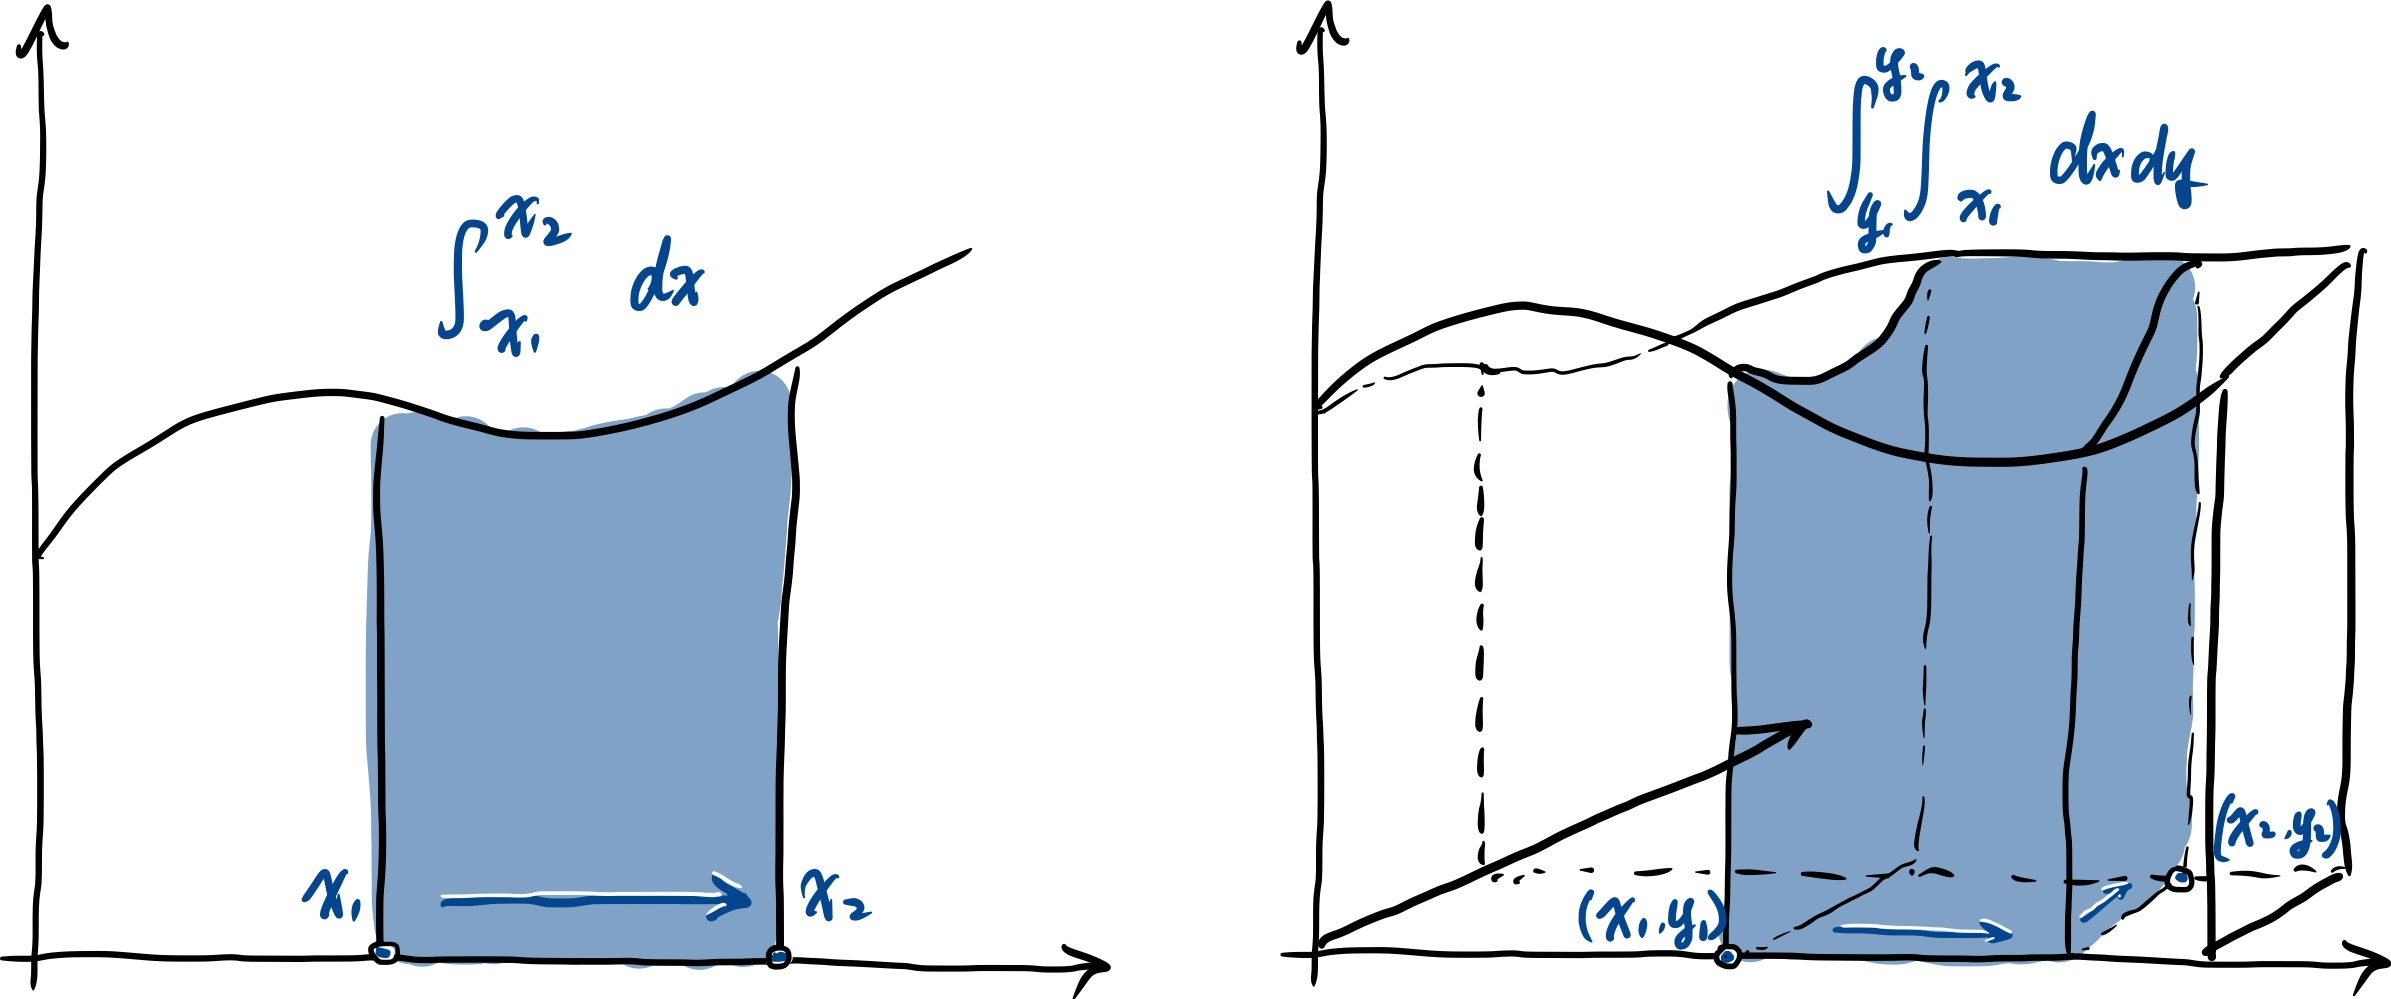
\includegraphics[width=0.9\textwidth]{./img/image-20240530065714806.png}
\end{tcolorbox}

对于三重积分, 我们可以参考前面的,
把它理解成一个三维``超曲面''在四维的空间中下方的四维``超体积'',
或者换一个思路, 我们可以考虑一个密度不均匀的三维物体,
其密度关于位置的函数给定, 已知其形状 (建立坐标系,
其形状可以用于决定积分的上下限) 的情况下, 它的质量就是一个三重积分
(回顾【\ref{019}\nameref{019}】文末).

\subsection{线积分}

英语中, 线积分 line integral 也常叫做 path integral, 可以直译作路径积分,
虽然比较直观, 但是可能和量子场论中的路径积分混淆,
所以下文还是统一做线积分. 顾名思义, 在不止一维的情况下,
对一个多元函数的积分从一个点到另一个点, 可以不止一条曲线 (路径),
所以线积分都需要 specify 积分的曲线. 线积分可能有以下几种 \[
\begin{aligned}
&\text{(i)}\ \ \int f\ \mathrm{d}\boldsymbol{r},\\
&\text{(ii)}\ \int\boldsymbol{v}\cdot\mathrm{d}\boldsymbol{r},\\
&\text{(iii)}\int\boldsymbol{v}\times\mathrm{d}\boldsymbol{r},
\end{aligned}
\] 分别是: (i) 标量场和一个``向量微元''的数乘的积分, (ii)
向量场和``向量微元''点乘的积分, (iii) 向量场和``向量微元''叉乘的积分
(三种情况如下图所示). 这里将 $\mathrm{d}\boldsymbol{r}$
称作``向量微元''并不是一个准确的描述, 通常来讲,
上述的积分都是沿着一条曲线, 所以 $\mathrm{d}\boldsymbol{r}$
作为这条曲线的一段无穷小量, 应该是切于这条曲线的一个向量 (切向量 -
tangent vector, 微分几何警告!).

\begin{tcolorbox}[size=fbox, breakable, enhanced jigsaw]
    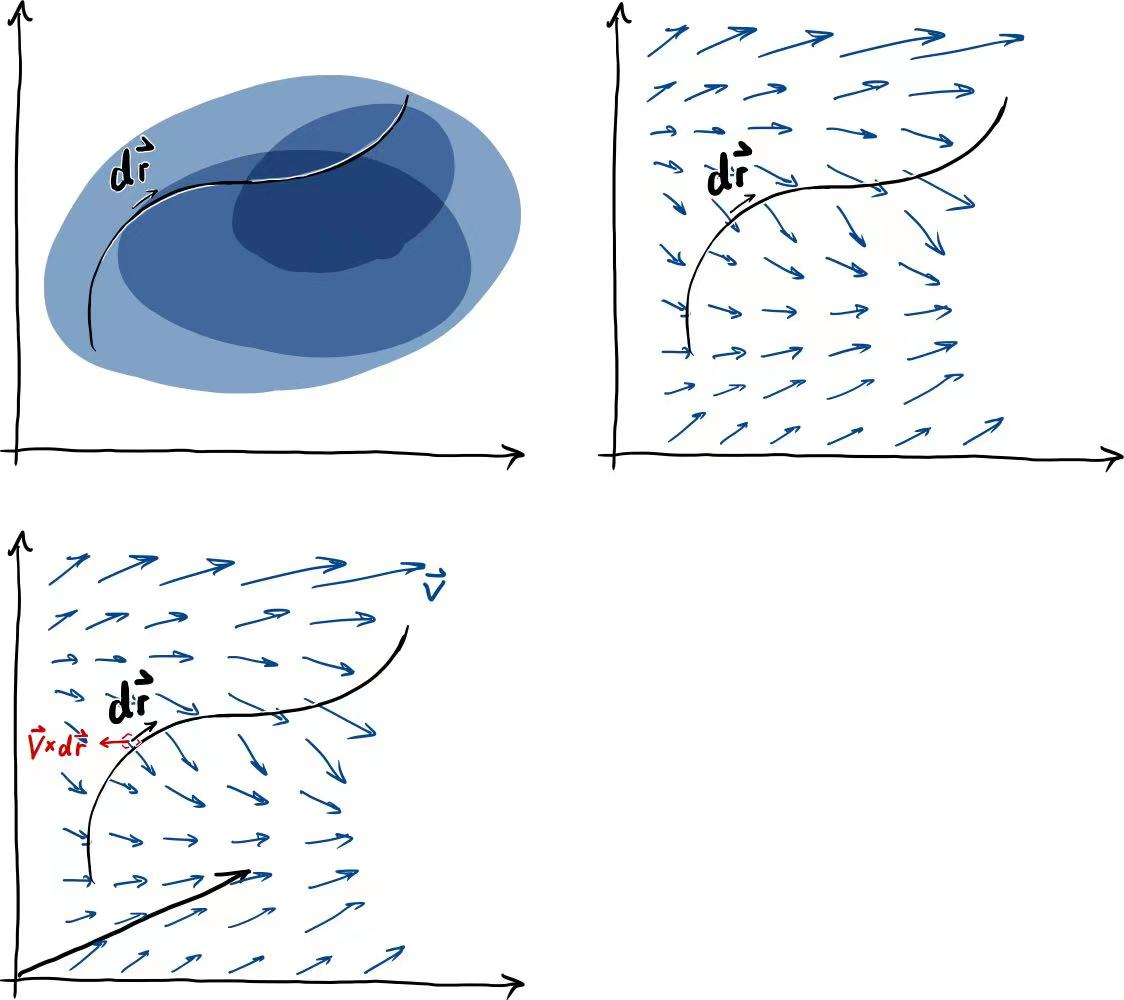
\includegraphics[width=0.9\textwidth]{./img/image-20240530065850401.png}
\end{tcolorbox}

\textbf{(i)}

考虑三维欧氏坐标系, 第一个积分可以展开作 \[
\int f\ \mathrm{d}\boldsymbol{r}=\int f(x,y,z)\mathrm{d}x\ \hat{\imath}+\int f(x,y,z)\mathrm{d}y\ \hat{\jmath}+\int f(x,y,z)\mathrm{d}z\ \hat{k},
\] 注意展开后的每一个积分, 以第一个关于 $x$ 的积分为例,
因为积分曲线是确定的, 所以 $\{y,z\}$ 不能被视作常数,
因为积分曲线已经给定, 比如以一个参数方程的形式: \[
\begin{cases}
x=x(t)\\
y=y(t)\\
z=z(t)
\end{cases},
\] 上式可以被改写为 $\{y(x),z(x)\}$, 于是在这条曲线上 $f$
可以被表述为仅关于 $x$ 的形式, 便可以对 $x$ 进行积分, 后两项也类似.
最后的结果应该是一个向量, 每一项积分的结果对应一个方向上的分量.

\begin{newquote}
考虑一条可以忽略横截面积的、密度不均匀的绳,
若其单位长度的质量以一标量场给出, 那么上述积分可以描述其质量.
\end{newquote}

\textbf{(ii)}

第二个积分是比较\textbf{常见}的, 和前面一样展开有 \[
\int\boldsymbol{v}\cdot\mathrm{d}\boldsymbol{r}=\int v_x(x,y,z)\mathrm{d}x+\int v_y(x,y,z)\mathrm{d}y+\int v_z(x,y,z)\mathrm{d}z,
\] 因为欧式坐标系中单位向量的正交归一性 (类似
$\hat{\imath}\cdot\hat{\imath}=1, \hat{\imath}\cdot\hat{k}=0$,
复习【\ref{025}\nameref{025}】), 只有上面三项是通常而言非零的, 其中 $\{v_x,v_y,v_z\}$
表示 $\boldsymbol{v}$ 的分量. 最后的结果应该是一个标量.

物理上常有做功的计算, 比如将一质点在一力场 $\boldsymbol{F}(x,y,z)$ 中,
沿一轨迹 $C(x,y,z)$ 移动, 做功便是 \[
W=\int_C\boldsymbol{F}\cdot\mathrm{d}\boldsymbol{r},
\] 其中积分符号下的 $C$ 强调积分曲线是 $C(x,y,z)$,
因为通常而言做功的大小是路径相关 (path dependent) 的,
也就是说即便是积分两端点一致, 不同的积分曲线得到的结果也会不一样.

\textbf{(iii)}

第三个积分可以展开作:

\[
\begin{aligned}
&\int\boldsymbol{v}\times\mathrm{d}\boldsymbol{r}\\
=&\int\begin{vmatrix}\hat{\imath}&\hat{\jmath}&\hat{k}\\v_x&v_y&v_z\\\mathrm{d}x&\mathrm{d}y&\mathrm{d}z\end{vmatrix}\\
=&\left(\int v_y\mathrm{d}z-\int v_z\mathrm{d}y\right)\hat{\imath}\\
&+\left(\int v_z\mathrm{d}x-\int v_x\mathrm{d}z\right)\hat{\jmath}\\
&+\left(\int v_x\mathrm{d}y-\int v_y\mathrm{d}x\right)\hat{k},
\end{aligned}
\]

叉乘不那么直观, 这样的线积分现实中也出现的较少,
但还是有一些用得到的例子.

\begin{newquote}
说到叉乘就想到右手定则 (复习【\ref{026}\nameref{026}】),
说到右手定则就想到了毕奥-萨伐尔定律 (Biot-Savart Law), which states that
\[
\boldsymbol{B}=\frac{\mu_0I}{4\pi}\int_C\frac{\mathrm{d}\boldsymbol{l}\times \boldsymbol{r}}{r^3},
\] 上式描述了通电导线产生的磁场 $\boldsymbol{B}$, $\mu_0$ 是一个常数
(真空磁导率), $I$ 是电流的大小, $\mathrm{d}\boldsymbol{l}$
是电流所在的线元, $\boldsymbol{r}$ 是线元指向待求磁场强度所在的点
(空间上我们关注的点, 在这个点上磁场强度是 $\boldsymbol{B}$), $r$ 是
$\boldsymbol{r}$ 的大小 (也就是线元到关注点的距离).

注: 其实上式中, 磁场和距离平方成反比 (i.e.~$B\propto1/r^2$), 磁场
$\boldsymbol{B}$ 的方向同时垂直于 $\boldsymbol{r}$ 和
$\mathrm{d}\boldsymbol{l}$, 所以叉乘只是希望得到磁场的方向, 但是
$\boldsymbol{r}$ 会额外 introduce 一个 $r=|\boldsymbol{r}|$ ,
所以为了消掉这个额外的 $r$, 分母便成了 $r^3$.
这也是库仑力或引力的向量公式里出现 $\boldsymbol{r}/r^3$ 的原因.
在一些记号中, 规定单位向量 $\hat{r}:=\boldsymbol{r}/r$
也可以使得公式看起来更自然, 当然也有教材使用 $\hat{e}_r$.
\end{newquote}

\subsection{面积分}

面积分也可以有几种情况: \[
\begin{aligned}
&\text{(i)}\ \ \int f\ \mathrm{d}\boldsymbol{a},\\
&\text{(ii)}\ \int\boldsymbol{v}\cdot\mathrm{d}\boldsymbol{a},\\
&\text{(iii)}\int\boldsymbol{v}\times\mathrm{d}\boldsymbol{a},
\end{aligned}
\] 稍难理解一些的是, 为什么面积会是一个向量; 事实上, 记
$a=|\boldsymbol{a}|$, 那么有
$\mathrm{d}\boldsymbol{a}=\hat{n}\mathrm{d}a$, 其中 $\hat{n}$
是面积元 $\mathrm{d}a$ 处的法向量 (normal vector). 对于一个闭曲面
(closed surface), 一般将向``外''记作法向量的正方向, 对于不封闭的单连通
(simply connected, 简单来说就是没有``洞'') 曲面 $S$,
若是给定曲面的边界 $\partial S$ (boundary) 的指向,
便可以用右手定则来决定法向量的方向.

\begin{newquote}
超纲\&剧透: 至于为什么曲面边界可以用偏导来表示, 需要一些外积, 外微分,
和微分形式的知识 (目前暂时只有在【\ref{026}\nameref{026}】的选读提及了一下外积), but in
short, generalized 的斯托克斯定律 (Stokes' theorem) 告诉我们 \[
\int_{\partial S}\omega=\int_S\mathrm{d}\omega,
\] 这里 $\omega$ 是待积分的微分形式.
狭义一点的版本的斯托克定律会在稍后呈现.
\end{newquote}

第 (ii) 个积分比较常用, 通常用来计算流量或者通量,
例如计算一个置于非匀强磁场中的环形电路围成的面积里的磁通量,
点乘的性质很好的解决了当磁感线与面积元不垂直的情况.

\subsection{体积分}

体积分大多数时候将体积元视作标量 $\mathrm{d}V$, 于是情况无非为: \[
\begin{aligned}
&\text{(i)}\ \ \int f\ \mathrm{d}V,\\
&\text{(ii)}\ \int\boldsymbol{v}\ \mathrm{d}V,
\end{aligned}
\] 通常第一个积分会比较常用, 例如已知一个物体的密度关于位置的函数,
待求这个物体的质量.

\begin{newquote}
实际上, 从外积的角度出发, 考虑三维欧氏空间中的一个平行于 $x-y$
平面的面元 $\mathrm{d}\boldsymbol{a}$ 可以写作
$(\mathrm{d}x\wedge\mathrm{d}y)$; 那么体元是不是就是
$(\mathrm{d}x\wedge\mathrm{d}y\wedge\mathrm{d}z)$ 了呢? 是也非也,
如果我们视体元为标量的化, 应该有
$\mathrm{d}V=|\mathrm{d}x\wedge\mathrm{d}y\wedge\mathrm{d}z|$,
但其实定义一个``向量''版本的体元也并非不可,
其几何含义可以仿照这二维面元, 解读为:
一个三维形状可以视作一个四维空间中的一个超曲面 (hypersurface),
于是向量体元 $(\mathrm{d}x\wedge\mathrm{d}y\wedge\mathrm{d}z)$
实际上是 $\mathbb{R}^4$ 中的一个``超曲面元''.

这样既然有了向量版本的体元, 便可以有它与向量场的点乘叉乘了 (我们日常的
$\mathbb{R}^3$ 大概是鲜有情况需要用到这一点,
不过很多利用到高维向量的学科, 例如机器学习中的支持向量机等,
类似的无用的知识点大概也许可能有点作用).
\end{newquote}
